\section{Ergebnisse}

\subsection{Zahlen ohne Optimierung}
Beim ersten Zoom ist ein 16-facher Zoom nicht mehr möglich, da die Matrix so gross wird, dass es nicht genügend RAM freiräumen kann. Ebenfalls dauert es dann schnell mal viel Zeit, einen 12-fachen Zoom mit der Auflösung 4'001 auf 2'667 Pixel zu berechnen, zum Punkt -1.25 und mit 150 Iterationen etwa 45.6 Stunden.\\
Durch die CUDA-Optimierung kann man nur noch einen 6.25-fachen Zoom machen, dies liegt daran das die GPU nur noch 8GB VRAM hat und der PC 16GB RAM. Bei gleicher Einstellung, bis auf die Zoomtiefe auf 6.25 konnte das Programm innerhalb von 38 Sekunden fertig rechnen. Dass ein Zoom nicht gleich tief möglich ist, ist eigentlich egal, denn es geht ja darum, die Rechenleistung zu verringern und einen allfälligen Algorithmus zu finden. Das gleiche Programm, ein 1-facher Zoom, dauert nun anstelle von 3 Stunden nur noch 2 Minuten.
\subsection{Analyse Ergebnisse}
\begin{figure}[!h]
	\centering
	\subfloat[1. Quadrant]{\scalebox{1}[-1]{\includegraphics[width=.49\textwidth]{Pictures/1AnalyBuddhabrotmengeWithZoomGPU1ToPoint-0.5 + 0.0imWithIteration1000withResolution4000x2667.png}}\label{fig:1. Quadrant}}
	\hfill
	\subfloat[2. Quadrant]{\scalebox{1}[-1]{\includegraphics[width=.49\textwidth]{Pictures/2AnalyBuddhabrotmengeWithZoomGPU1ToPoint-0.5 + 0.0imWithIteration1000withResolution4000x2667.png}}\label{fig:2. Quadrant}}
	\hfill
	\subfloat[3. Quadrant]{\scalebox{1}[-1]{\includegraphics[width=.49\textwidth]{Pictures/3AnalyBuddhabrotmengeWithZoomGPU1ToPoint-0.5 + 0.0imWithIteration1000withResolution4000x2667.png}}\label{fig:3. Quadrant}}
	\hfill
	\subfloat[4. Quadrant]{\scalebox{1}[-1]{\includegraphics[width=.49\textwidth]{Pictures/4AnalyBuddhabrotmengeWithZoomGPU1ToPoint-0.5 + 0.0imWithIteration1000withResolution4000x2667.png}}\label{fig:4. Quadrant}}
\caption{Das Buddhabrot der einzelnen Quadranten}
\end{figure}
\begin{figure}[h!]
	\centering
	\subfloat[1. Quadrant]{\scalebox{1}[-1]{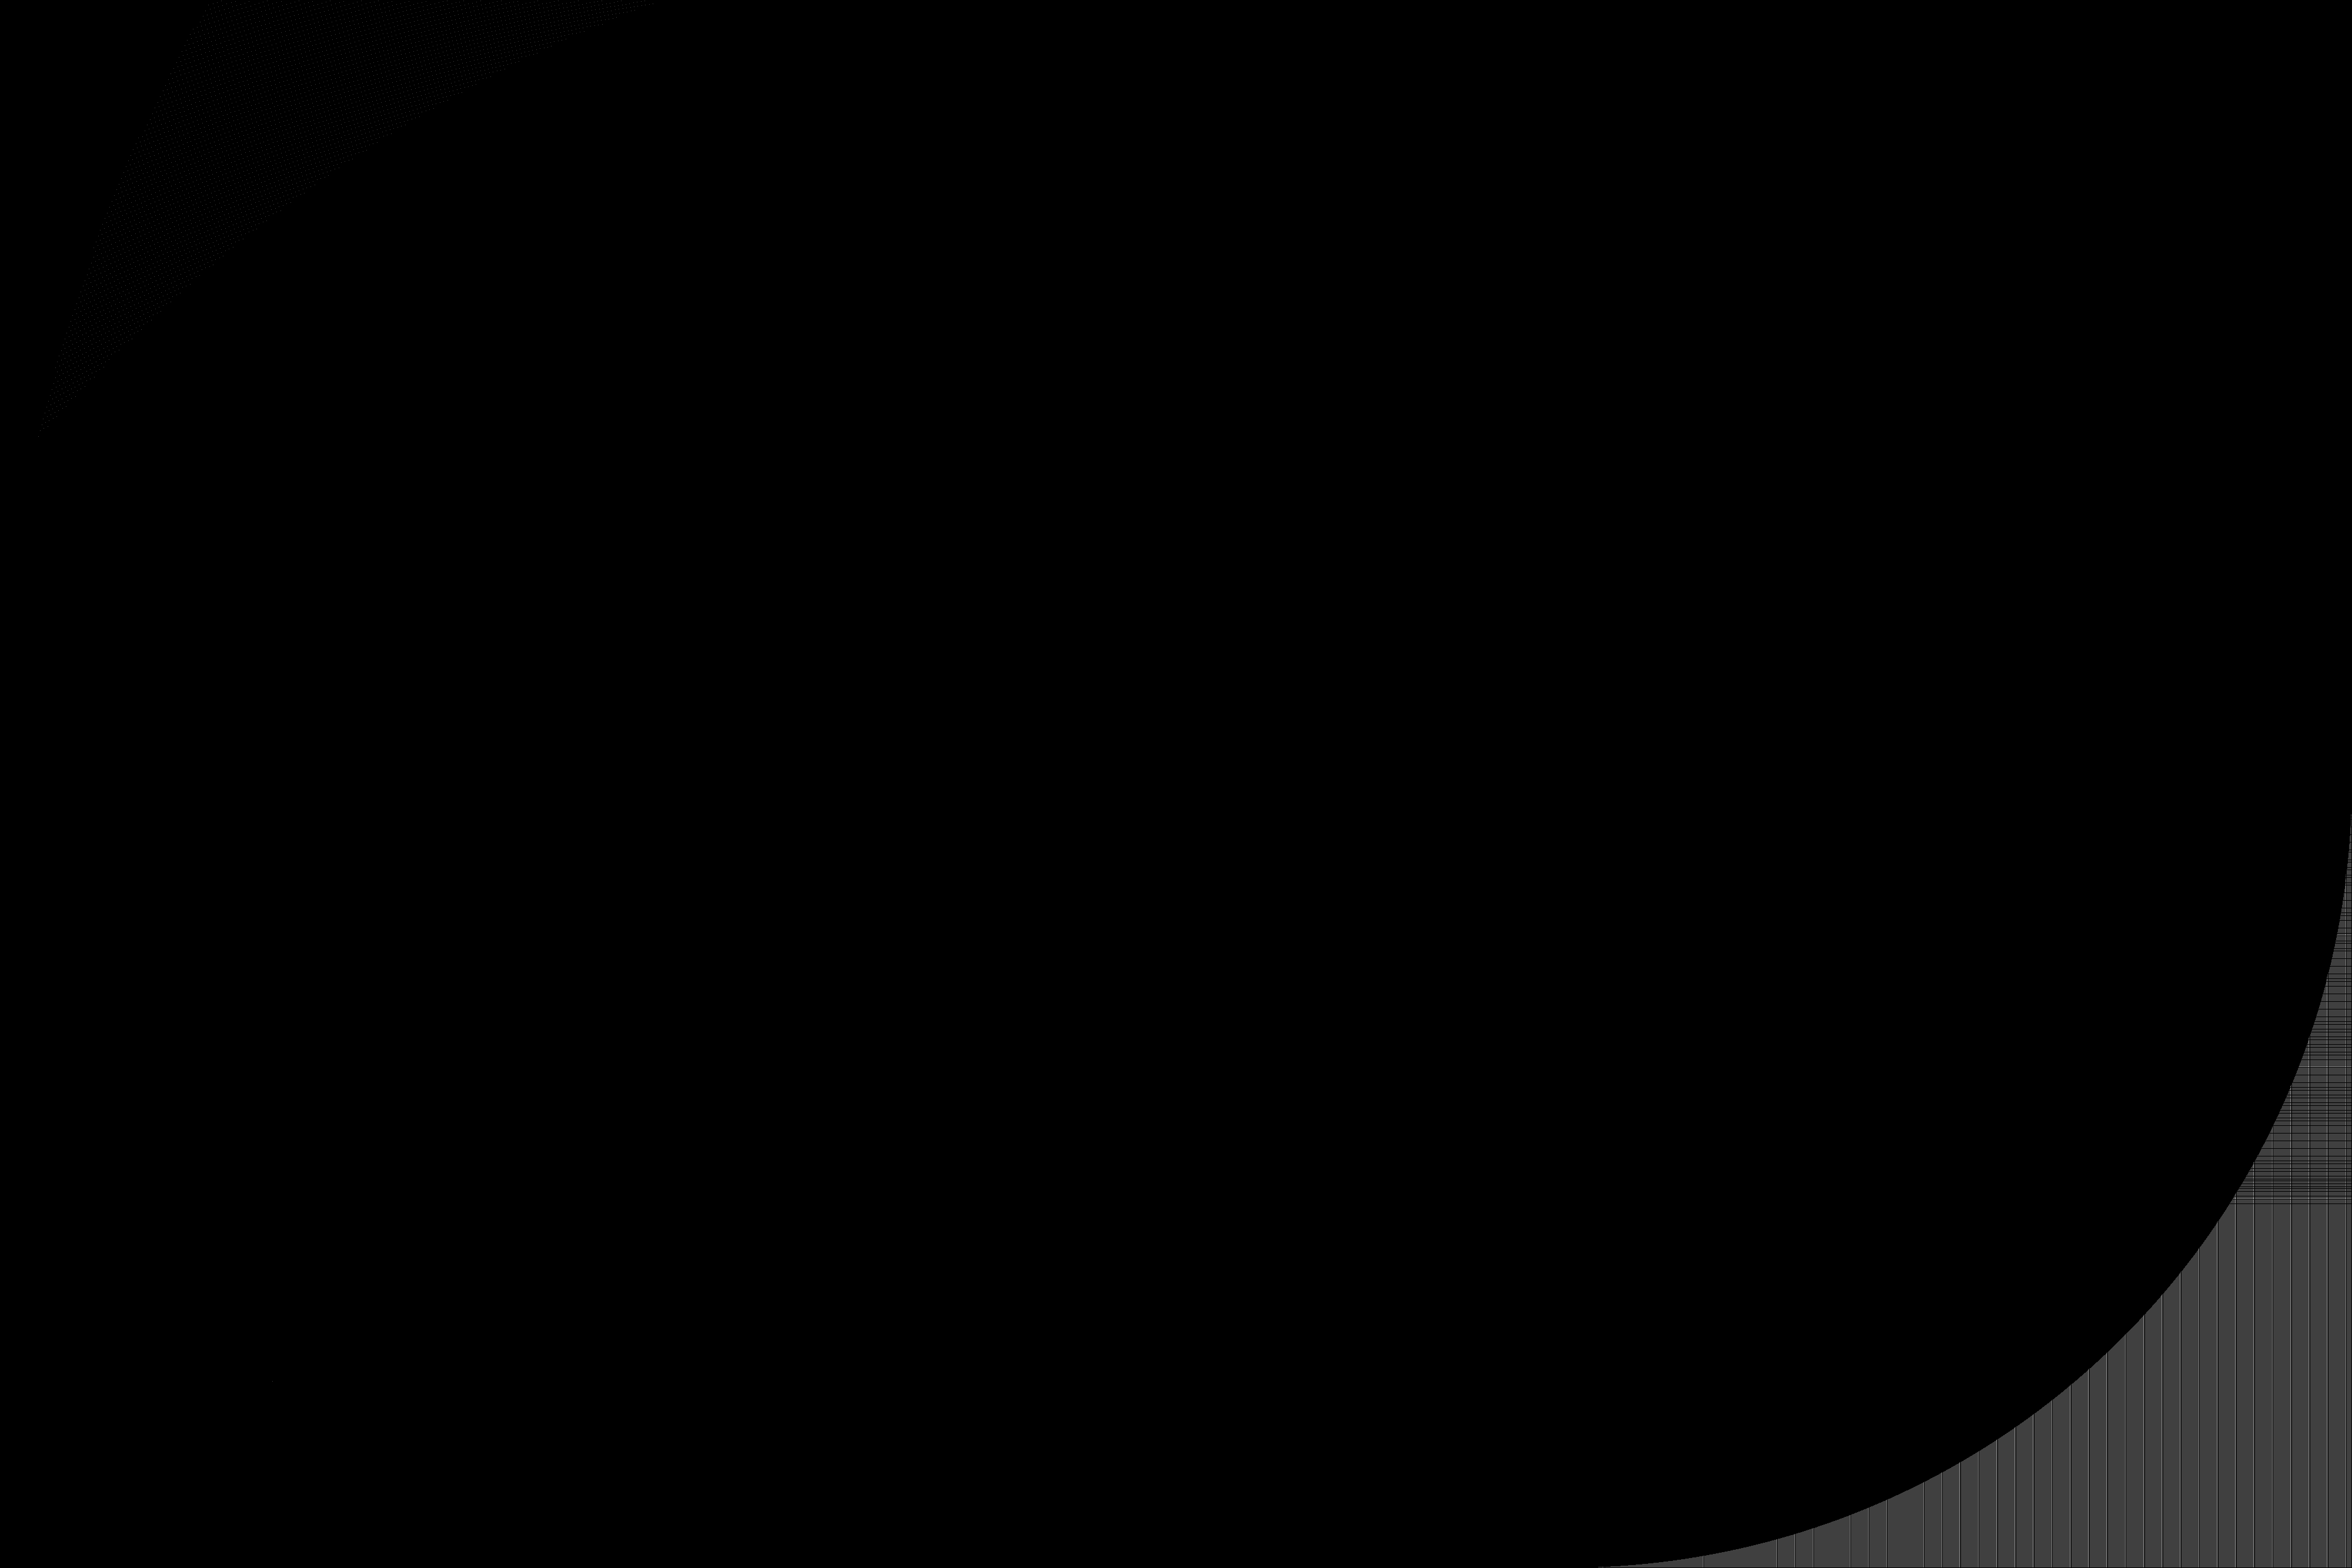
\includegraphics[width=.49\textwidth]{Pictures/10AnalyBuddhabrotmengeWithZoomGPU1ToPoint-0.5 + 0.0imWithIteration10000withResolution4000x2667.png}}\label{fig:1. Quadrant, abs}}
	\hfill
	\subfloat[4. Quadrant]{\scalebox{1}[-1]{
\includegraphics[width=.49\textwidth]{Pictures/40AnalyBuddhabrotmengeWithZoomGPU1ToPoint-0.5 + 0.0imWithIteration10000withResolution4000x2667.png}}\label{fig:4. Quadrant, abs}}
	\caption{Das Buddhabrot für $\{z \in \mathbb{C}| |z|>1\}$ in den Quadranten 1 \& 4}
	\label{fig:absolute}
\end{figure}
Bei Abbildung \ref{fig:absolute} ist der maximal erreichte Treffer auf einem Pixel vier.

\subsection{Implementierungszahlen}
Durch die gefundene Lösung ist ein 6.48-facher Zoom möglich, jedoch braucht ein gleicher Zoom mehr Zeit. Dies liegt daran, dass nun grosse Matrixen in einer Liste zu finden sind und so der Aufruf durch mehrere if-Kondition länger dauert. Es ist jedoch ein minimaler Verlust und somit nicht schlimm. Ein 6.48-facher Zoom zum Punkt -1.25, mit der Auflösung 4'002 auf 2'668 Pixel und mit 100 Iteration dauert es nur noch 2 Minuten und 10 Sekunden. Bei einem 6.25-fachem Zoom braucht es 2 Minuten 1 Sekunde.
